\Chapter{Approximations de l'équation de quantité de mouvement}
\chaptermark{Approx. de l'équation de quantité de mouvement}

\label{ApproximationsEqMvt}
\begin{refsection}
Dans ce chapitre, nous présentons deux modèles courament utilisés 
pour décrire les plasmas magnétisés. Le modèle de dérive-diffusion utilisé dans
le domaine des plasmas froids, suppose un plasma collisionnel et stationnaire.
Le modèle des vitesses de dérive représente des plasmas totalement ionisés et très
magnétisés. Nous discutons enfin de la pertinence des deux modèles dans le cadre
de la modélisation des sources basse-pression.

\section{L'équation de quantité de mouvement}

Dans sa vocation à expliquer et comprendre les phénomènes naturels et les
systèmes complexes, la recherche scientifique se base toujours sur la
formalisation des concepts, des processus et des interactions dans des
modèles, représentations intelligibles de la réalité. En physique, ces modèles
peuvent être plus ou moins complets ou simplifiés en fonction des hypothèses
initiales et des différentes approximations. Ils ne sont
pas censés représenter exactement leur sujet, mais au moins décrire une
certaine physique mise en jeu.
Les modèles sont l'un des
principaux outils de la science moderne, et, grâce à l'outil numérique, nous
donne accès à une réalité virtuelle plus facilement analysable et questionnable
que le vrai monde.

\begin{figure}[!htbp]
    \centering
	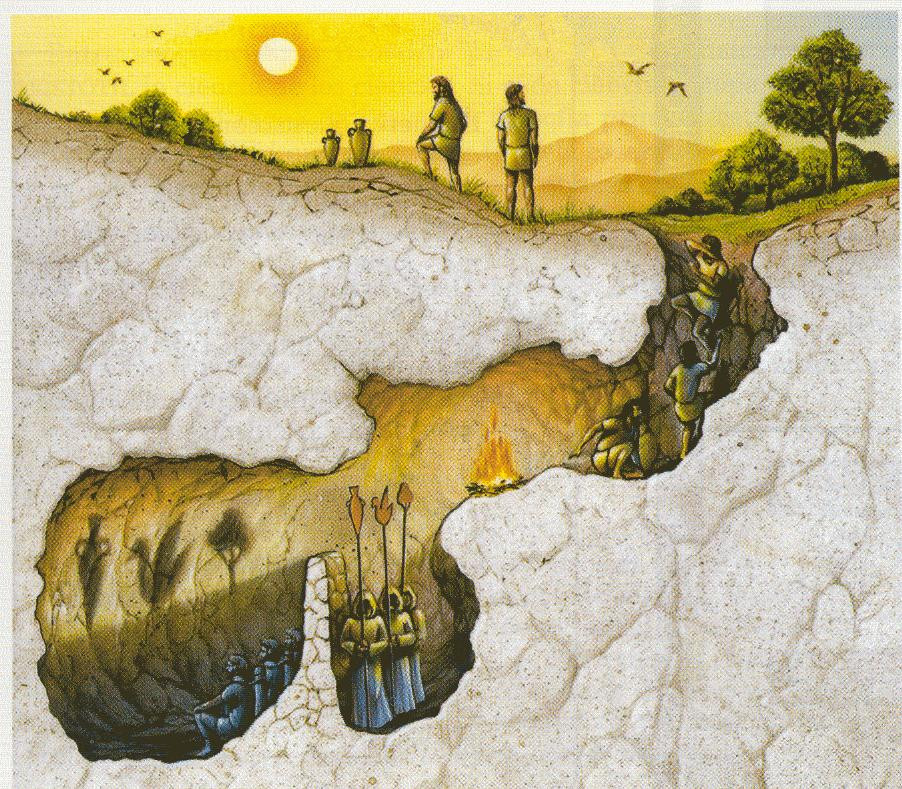
\includegraphics[width=0.5\textwidth]{figures/1-cave.jpg}
	\caption{Allégorie de la caverne. La célèbre histoire de
	Platon~\parencite{Platon} raconte l'histoire d'hommes condamnés à ne voir que
	l'apparence des phénomènes qui les entourent. Afin de parvenir à la connaissance de la réalité
	intelligible des Idées, ils doivent effectuer une démarche intellectuelle
	et sortir de la caverne.}\label{caverne}
\end{figure}


Actuellement, les modèle les plus complets pour décrire un plasma sont sans
conteste les modèles cinétiques. Cependant, en plus d'être très coûteux à
résoudre numériquement, ces modèles donnent des résultats très bruités
et difficilement interprétables. Pour la compréhension des phénomènes qui ont
lieux dans les plasmas, on leur préfère donc assez souvent un modèle fluide, qui
donne un accès plus direct aux mécanismes de transport. En fonction des
processus et des phénomènes de transport que l'on désire observer, les modèles
fluides, qui permettent d'isoler, de négliger, ou même d'amplifier certains
termes, sont plus à même de nous aider à comprendre les liens entre les différents mécanismes.

Dans la théorie fluide, l'équation de quantité de
mouvement \eqref{1-eqMouvement}, qui contrôle l'évolution des vitesses fluides
$\mathbf u_\alpha$, régit l'essentiel de la dynamique du plasma. Cependant, comme sa forme complète
 est encore trop compliquée, il est courant de la
simplifier davantage en considérant d'autres hypothèses.
La première de ces hypothèses communément retenue pour simplifier l'équation de
la quantité de mouvement consiste à considérer le tenseur de pression isotrope,
ie.
$\boldsymbol{\Pi}_\alpha=0$, en supposant que les transferts d'impulsion dus
aux collisions entre particules d'espèces différentes ont plus d'effet que
ceux résultants de la viscosité. L'équation de la quantité de
mouvement~\eqref{1-eqMouvement} se réduit ainsi à un équilibre entre les forces
d'inertie, de frottement, de Lorentz et de pression :

\begin{equation}
\label{1-eqBilanForce}
\underbrace{m_\alpha \left(\partial_t \mathbf{u_\alpha} +
(\mathbf{u_\alpha}\cdot\nabla)\mathbf{u_\alpha}\right)}_\text{Inertie}
+\underbrace{m_\alpha\left(\nu_\alpha^c+
\nu_\alpha^\text{iz}\right)\mathbf
u_\alpha}_\text{Frottement \& Création}=\underbrace{{q_\alpha}\left(\mathbf
E+\mathbf u_\alpha\times \mathbf B\right)}_\text{Forces électromagnétiques}
-\underbrace{\frac{\nabla p_\alpha}{n_\alpha}}_\text{Pression}
\end{equation}
 
Le poids des différents termes de \eqref{1-eqBilanForce} varie en fonction des
paramètres du plasma et permet de définir les types de mécanismes qui régissent
le transport des fluides électroniques et ioniques. Les termes estimés petits
relativement aux autres peuvent ainsi être négligés pour obtenir une
expression plus simple de la vitesse fluide et permettre des développements
analytiques.

Un premier cas limite peut être obtenu quand le terme de pression domine
sur l'ensemble des termes du membre de gauche de \eqref{1-eqBilanForce}. Ce cas
de figure est caractéristique pour des électrons non-collisionnels enfermés
dans un puit de potentiel (par exemple résultant de l'interaction entre le
plasma et les parois). Dans ces conditions, \eqref{1-eqBilanForce} s'écrit:

\begin{equation}
\label{1-equilibreBoltzman}
q_\alpha\mathbf
E =\frac{e}{n_\alpha}\nabla n_\alpha T_\alpha
\end{equation}

C'est la relation de Boltzmann, qui s'obtient généralement en intégrant la
distribution de Maxwell-Boltzmann :

\begin{equation}
\label{1-profilBoltzman}
n_\alpha=\frac{n_0}{H^2\left(2T_e/m_e\right)^{3/2}}\exp(-\frac{\mathcal
U - e\Phi}{T_\alpha})
\end{equation}

En l'absence de champ magnétique ou parallèlement aux lignes de champ, le champ
électrique et le gradient de pression se compensent. Cette hypothèse est
fondamentale dans la dérivation des modèles fluides de transport pour les plasmas dans la mesure où elle constitue l'une des bases de
la théorie des gaines vue précédemment. 

Dans le domaine des plasmas
froid, on fait l'hypothèse de forte collisionnalité et on développe
l'équation de la quantité de mouvement en fonction du petit paramètre
$\lambda_{lpm}/L$.
Dans le domaine des plasmas de fusions fortement magnétisés, il est
plutôt d'usage de considérer le petit paramètre $\delta=\rho_L/L$ pour moyenner
l'équation \eqref{1-eqBilanForce} sur les échelles de temps supérieures à
l'inverse de la fréquence cyclotronique $\omega_{c}$.


\section{Cas collisionnel : Équation de dérive-diffusion}
\label{1-transportAmbipolaire}
\subsection{Équation de dérive-diffusion non magnétisée}
Les plasmas froids de décharge utilisés dans l'industrie et la recherche n'ont
en général qu'un faible degré d'ionisation $\alpha<$1\% et la dynamique des
espèces y est dominée par la perte de quantité de mouvement liée à l'ionisation
et aux collisions avec le gaz. Pour modéliser ce type de plasma, la prise en
compte du terme collisionnel dans l'équation de la quantité de mouvement est
essentielle.
En l'absence de champ magnétique, le rapport d'échelle entre le libre parcours moyen des particules
et la taille du plasma $\lambda_\alpha\ll L$ permet de simplifier l'équation de
la quantité de mouvement en négligeant les termes d'inertie, relativement
faibles par rapport au terme collisionnel :

\begin{equation}
\label{1-eqDriftDif}
n_\alpha\mathbf u_\alpha=\frac{q_\alpha}{\nu_\alpha m_\alpha}n_\alpha\mathbf
E-\frac{\nabla\left(n_\alpha T_\alpha\right)}{\nu_\alpha
m_\alpha}
\end{equation}

avec $\nu_\alpha=\nu_\alpha^c+\nu_\alpha^\text{iz}$ une fréquence de collision
effective. Dans le cas d'un plasma isotherme, on peut sortir la température de
la divergence.
En notant $\mu_\alpha=e/\nu_\alpha m_\alpha$ et
$D_\alpha=T_\alpha/\nu_\alpha m_\alpha$, le flux de \eqref{1-eqDriftDif} se
réécrit avec une loi d'Ohm et une loi de Fick :

\begin{equation}
\label{1-eqDriftDif2}
n_\alpha\mathbf u_\alpha\equiv\underbrace{\frac{q_\alpha}{|q_\alpha|}\mu_\alpha n_\alpha\mathbf E}_\text{Loi d'Ohm}+\underbrace{D_\alpha{\nabla n_\alpha}}_\text{Loi
de Fick}
\end{equation}

 C'est le flux de dérive-diffusion, caractérisé par les coefficients de
transport $\mu_\alpha$ et
$D_\alpha$, tous deux inversement proportionnels à la fréquence de collision
$\nu_\alpha$ (donc à la densité de gaz), et reliés par la relation d'Einstein :

\begin{equation}
\label{1-EinsteinRelation}
D_\alpha/\mu_\alpha=\frac{T_\alpha}{e}
\end{equation}

\begin{itemize}
  \item la mobilité, définie par $\mu_\alpha$,
  mesure la disposition d'une espèce à laisser passer le courant au sein d'un milieu
  \item la diffusion, de coefficient $D_\alpha$,
  représente la tendance naturelle d'un système à rendre homogène sa densité de particule sous l'effet
  de l'agitation thermique.
\end{itemize}

En combinant \eqref{1-eqDriftDif2} avec l'équation de continuité
\eqref{1-eqContinuite}, on obtient l'équation d'évolution de la densité
dite de dérive-diffusion :
 
\begin{equation}
\label{1-eqDriftDifContinuite}
\partial_t
n_\alpha=\nabla\cdot({\frac{q_\alpha}{|q_\alpha|}\mu_\alpha n_\alpha\mathbf E}
+{D_\alpha{\nabla n_\alpha}})+S_\alpha
\end{equation}

Dans des plasmas de décharge collisionnels, à partir de la source d'ionisation,
les électrons ont tendance à se déplacer beaucoup plus rapidement que les ions
du fait de leur faible masse et de leur température. Cette différence de
mobilité entraîne l'apparition d'un champ électrique dit "ambipolaire"
$\mathbf E_a$, faisant dériver les ions et les électrons ensembles et
systématiquement dirigé dans le sens opposé du gradient de densité afin de
limiter la diffusion des électrons et accélérer les ions. En ne considérant
qu'une seule espèce ionique, on trouve son expression en cherchant le champ
correspondant à un courant nul :
 
\begin{equation}
\label{1-eqEAmb}
\mathbf j=0 \Rightarrow \mathbf E=\mathbf
E_a=\frac{D_i-D_e}{\mu_i+\mu_e}\frac{\nabla
n}{n}
\end{equation}

Si l'on applique l'équation de
dérive-diffusion~\eqref{1-eqDriftDifContinuite} à un plasma peu collisionnel,
ie. dans la limite $\nu_{i,e}\rightarrow\,$0, cette description peut poser
problème, les mobilités tendant quant à elles vers l'infini. Le modèle de
dérive-diffusion n'est en effet strictement valide que quand le libre parcours
moyen ne dépasse pas la longueur caractéristique des gradients $\lambda\sim L_{\nabla}$. 

Quand ce critère n'est pas respecté, ce n'est pas très grave pour les
électrons, l'équilibre de
Boltzmann tenant toujours.
Pour les ions, la seule issue repose sur la prise en compte du
terme de création $\nu^\text{iz}_i\mathbf u_i$ qui défini une limite haute pour
la mobilité ionique.
Le modèle de dérive-diffusion est ainsi encore utilisable, mais perd beaucoup en
précision.

Regardons maintenant ce que donne ce modèle en présence d'un champ magnétique.

\subsection{Équation de dérive-diffusion magnétisée}
\label{1-deriveDiffMag}
L'utilisation d'un champ magnétique dans un plasma permet de contrôler en partie
le transport des particules et d'obtenir des configurations favorables pour
diverses applications. Cependant, la prise en compte du terme de Laplace dans
\eqref{1-eqBilanForce} impose une forte anisotropie dans le système, ce qui
complexifie considérablement les phénomènes de transport. En
négligeant l'inertie, on peut considérer \eqref{1-eqBilanForce} comme une
équation algébrique d'inconnue $\mathbf u$ ; le réagencement des différents
termes donne :

\begin{equation}
\label{2-eqDriftDifMag}
\begin{split}
n_\alpha\mathbf u_\alpha&=\frac{q_\alpha}{|q_\alpha|}\mu_\alpha
n_\alpha\left(\mathbf E+\mathbf u_\alpha\times\mathbf
B\right)-D_\alpha\nabla\left( n_\alpha\right)
\\
&=\frac{q_\alpha}{|q_\alpha|} n_\alpha\left(\mu_{\alpha_\para}\left(\mathbf
b\cdot\mathbf E\right)\mathbf b+\mu_{\alpha_\perp}\left(\mathbf
E-\left(\mathbf
b\cdot\mathbf E\right)\mathbf
b\right)+\mu_{\alpha_\times}\mathbf
b\times\mathbf E\right)
\\
&-\left(D_{\alpha_\para}\left(\mathbf
b\cdot\nabla n_\alpha\right)\mathbf b+D_{\alpha_\perp}\left(\mathbf
\nabla n_\alpha-\left(\mathbf
b\cdot\nabla n_\alpha\right)\mathbf
b\right)+D_{\alpha_\times}\mathbf
b\times\mathbf \nabla n_\alpha\right)
\end{split}
\end{equation}

Pour une meilleure lisibilité, on réécrit l'équation~\ref{2-eqDriftDifMag}
sous forme tensorielle, donnant l'équation de dérive-diffusion magnétisée,
courament utilisée dans le domaine des plasmas froids pour modéliser le
transport magnétisé~\parencite{grephe, propulseur} :

\begin{equation}
\label{2-eqDriftDifMag2}
n_\alpha\mathbf u_\alpha\equiv
\frac{q_\alpha}{|q_\alpha|} n_\alpha\boldsymbol{\mu}_\alpha\cdot \mathbf
E-\mathbf{D}_\alpha{\nabla\left( n_\alpha\right)}
\end{equation}

où la mobilité $\boldsymbol{\mu}_\alpha$ et la diffusion $\mathbf{D}_\alpha$
sont devenus des tenseurs d'ordre 2. Dans un repère avec le champ magnétique axé
sur la direction du champ magnétique $\mathbf B=B\mathbf e_z$ :

\begin{align}
\boldsymbol{\mu}_\alpha =
 \begin{pmatrix}
  \mu_{\alpha_\perp} & \pm\mu_{\alpha_\times} & 0 \\
  \pm\mu_{\alpha_\times} & \mu_{\alpha_\perp} & 0 \\
  0  & 0  & \mu_{\alpha_\para} 
 \end{pmatrix}\;\;\;\;\text{et}\;\;\;\;
 \mathbf D_\alpha =
 \begin{pmatrix}
  D_{\alpha_\perp} & \pm D_{\alpha_\times} & 0 \\
 \pm D_{\alpha_\times} & D_{\alpha_\perp} & 0 \\
  0  & 0  & D_{\alpha_\para} 
 \end{pmatrix}
\end{align}

Dans la direction parallèle au champ magnétique, les coefficients de mobilité et
de diffusion sont inchangés
$\mu_{\alpha\para}=\mu_{\alpha}=q_\alpha/m_\alpha\nu_\alpha$ et
$D_{\alpha\para}=D_\alpha=T_\alpha/m_\alpha\nu_\alpha$. Les coefficients de la
direction perpendiculaire font quant à eux apparaître le paramètre de Hall
$h_\alpha=\omega_{c\alpha}/\nu_\alpha$ :

\begin{align}
\mu_{\alpha\perp}=\frac{1}{1+h_\alpha^2}\mu_\alpha\;\;\;\;\;\;\;\;
\;\;\;\;D_{\alpha\perp}=\frac{1}{1+h_\alpha^2}D_\alpha
\end{align}
\begin{align}
\mu_{\alpha\times}=\frac{h_\alpha}{1+h_\alpha^2}\mu_\alpha\;\;\;\;
\;\;\;\;\;\;\;\;D_{\alpha\times}=\frac{h_\alpha}{1+h_\alpha^2}D_\alpha
\end{align}

Quand $h_\alpha=0$, les tenseurs sont diagonaux et isotropes. Ensuite, plus le
paramètre de Hall augmente, plus le transport dans les directions transverses se
réduit :
les coefficients indicés avec le symbole perpendiculaire sont inversement
proportionnels au carré du champ magnétique $\mu_{\alpha\perp},
D_{\alpha\perp}\propto B\puissance{-2}$ ; à partir de $h_\alpha=1$, le
transport croisé commence à dominer sur le transport collisionnel et devient proportionnel à
$B\puissance{-1}$. Cette loi de puissance que suit le transport par rapport au
champ magnétique est souvent interprétée comme la signature d'un transport
anormal, mais apparaît naturellement dans les équations à travers les
coefficients de transport $\mu_{\alpha\times}$ et $D_{\alpha\times}$.

Dans les sources magnétisées, pour un paramètre de Hall électronique de l'ordre
de $h_e\approx\,$1000, on obtient typiquement des ratios sur les modilités :

\begin{equation}
\frac{\mu_{e_\perp}}{\mu_{e_\para}}\approx
10^{-6}-10^{-10}\text{~~~~~~~~et~~~~~~~~}\frac{\mu_{e_\times}}{\mu_{e_\para}}\approx
\frac{\mu_{e_\perp}}{\mu_{e_\times}}\approx10^{-3}
\end{equation}

En revanche, les ions n'étant généralement que peu magnétisés, leur mobilité
dans la direction perpendiculaire reste principalement fonction de la fréquence
de collision et d'ionisation  :

\begin{equation}
\mu_{i_\times}=\frac{h_i}{1+h_i^2}\mu_i=\frac{e^2B}{(\nu_i^2+\omega_{ci}^2)}\propto\frac{1}{\nu_i^2}
\end{equation}

À travers le champ magnétique, les ions sont alors plus rapides que les
électrons, les deux fluides se séparent, entraînant l'apparition d'un
courant : le courant de Hall. 

\section{Approche par les vitesses de dérive}
\label{vitessesDerive}
L'approche par les vitesses de dérive est à la base de nombreux modèles
développés pour étudier le transport dans les plasmas de fusion par
confinement magnétique~\parencite{Garcia,Bisai,Tamain}. Dans cette approche, la
vitesse des particules est exprimée en fonction du mouvement cyclotronique rapide, d'une composante
parallèle au champ magnétique et d'une dérive lente du centre-guide des particules dans
la direction transverse. Cette décomposition, qui peut se voir comme une
version fluide de la théorie particulaire du centre-guide, sous-entend que les
fréquences cyclotroniques sont grandes devant les fréquences caractéristiques du
transport, ie. $\omega_{ce},\omega_{ci}\gg\omega$. 
 
\subsection{Les plasmas de la Scrape-Off-Layer}
La Scrape-Off-Layer des tokamaks, ou SOL, est la zone en
périphérie du plasma confiné, ie. qui commence à partir de la séparatrice et qui
peut éventuellement s'étendre jusqu'aux parois internes du tore (voir
figure~\ref{SOL}). Dans cette région, les
particules ne sont plus confinées car les lignes de champ interceptent un
obstacle matériel (un limiteur ou un divertor) traité et dessiné spécifiquement
pour supporter les flux de matière et de chaleur qui s'échappent du plasma de
c\oe ur par transport transverse.
En conséquence, les profils de densité et de température s'effondrent sur une
longueur caractéristique qui définit la largeur de la SOL, $\lambda_\text{SOL}$,
donnant naissance à de forts gradients qui maintiennent le plasma hors
de l'équilibre thermodynamique.

\begin{figure}[!htbp]
    \centering
	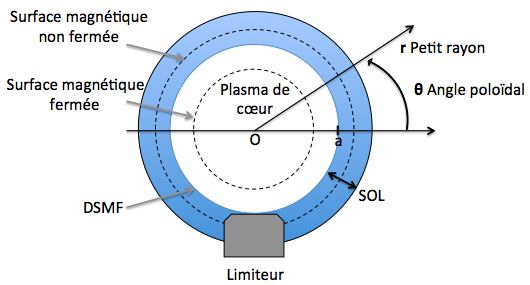
\includegraphics[width=0.8\textwidth]{figures/1-SOLLimiter.png}
	\caption{Coupe poloïdale du tokamak en configuration limiteur. De part et
	d'autre de la Dernière Surface Magnetique Fermée (DSMF située en r=a), le
	limiteur délimite le plasma de c\oe ur (r<a) de la SOL (r>a).}\label{SOL}
\end{figure}
 
Typiquement, les plasmas de SOL ont une densité de
l'ordre de 10$^{19}$~m$^{-3}$ et une température inférieure à la centaine
d'électronvolts. A cette température, le plasma est presque totalement ionisé et
le champ magnétique, d'environ 3T, confine efficacement les particules dans un
mouvement cyclotronique de fréquence $\omega_{ci}\sim45$~MHz pour un proton et
$\omega_{ce}\sim80$~GHz pour un électron, toutes deux bien supérieures à la
fréquence caractéristique du transport parallèle :

\begin{equation}
\omega_\para\sim
\frac{v_{\text{T}\alpha}}{L_\para}\approx\omega_{c\alpha}\frac{\rho_{L\alpha}}{L_\para}\rightarrow
\delta=\frac{\rho_{L\alpha}}{L_\para}=\frac{\omega_\para}{\omega_{c\alpha}}\ll1
\end{equation} 

Dans la direction perpendiculaire au champ
magnétique, les vitesses de dérive associées aux gradients transverses (dont les longueurs
typiques $L_\nabla$ de quelques centimètres sont bien supérieures aux rayon de
Larmor ionique $\rho_{Li}\approx3.10^{-4}$~m et électroniques
$\rho_{Le}\approx7.10^{-6}$~m) entraînent un transport de fréquence
caractéristique $\omega_\perp\sim v_\perp/L_\para\sim\rho_{L\alpha}
v_{\text{T}\alpha}/(L_\para L_\nabla)$ de deux ordres de grandeur inférieur à
$\omega_{c\alpha}$ :

\begin{equation}
\frac{\omega_\perp}{\omega_{c\alpha}}\approx\frac{\rho_{L\alpha}^2}{L_\para
L_\nabla}\sim\delta^2
\end{equation}

Malgré leur faible fréquence, ces vitesses de dérives sont à l'origine de tous
les mécanismes de micro-turbulence et jouent ainsi un rôle primordiale dans le
problème du confinement des plasmas de fusion.

\subsection{Vitesses de dérive électrique et diamagnétique}

Quand le degré d'ionisation du plasma est très élevé, le terme issu de
l'interaction avec le gaz peut être négligé dans l'équation de la quantité de
mouvement~\eqref{1-eqBilanForce} :

\begin{equation}
\label{1-eqSOL}
 m_\alpha n_\alpha\left(\partial_t \mathbf{u_\alpha} +
(\mathbf{u_\alpha}\cdot\nabla)\mathbf{u_\alpha}\right)
={q_\alpha n_\alpha}\left(\mathbf E+\mathbf
u_\alpha\times \mathbf B\right)
-{\nabla p_\alpha}
\end{equation}

 Sous l'hypothèse de faible variation spatiale des grandeurs et des champs à
 l'échelle du rayon de Larmor, la lente évolution du système par rapport aux
 fréquences cyclotroniques permet d'effectuer un développement de l'équation de
 la quantité de mouvement en fonction du petit paramètre $\delta$. En négligeant
 le mouvement cyclotronique, qui correspond à l'ordre 0 de ce développement et qui
 est de moyenne nulle sur un temps $t\sim\omega_{c\alpha}^{-1}$, la projection
 de~\eqref{1-eqSOL} perpendiculairement au champ magnétique s'écrit à l'ordre 1
 en $\delta$ :
 
 \begin{equation}
\label{1-eqSOLperp}
0
={q_\alpha n_\alpha}\left(\mathbf E+\mathbf
u_{\alpha\perp}^{(1)}\times \mathbf B\right)
-{\nabla_\perp p_\alpha}
\end{equation}

où $\mathbf E$ est le champ électrique dérivant du potentiel électrostatique
$\Phi$. En prenant le produit vectoriel par $\mathbf B$ de cette équation, on
obtient les deux vitesses de dérive fluides principales, la vitesse de dérive
électrique $\mathbf u_E$ et la vitesse de dérive diamagnétique $\mathbf u_*$,
respectivement liées aux gradients transverses de potentiel électrique $\Phi$ et
de pression $p_\alpha$:

\begin{equation}
\label{1-eqVitessesDerive}
\mathbf u_{\alpha\perp}^{(1)}=\mathbf u_E+\mathbf u_*=\frac{\mathbf
B\times\nabla_\perp \Phi}{B^2}+\frac{\mathbf B\times\nabla_\perp
p_\alpha}{n_\alpha q_\alpha B^2}
\end{equation}

\begin{figure}[!htbp]
    \centering
	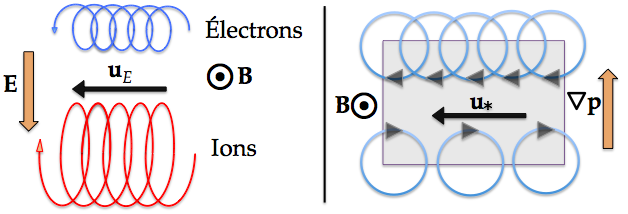
\includegraphics[width=0.9\textwidth]{figures/1-vitessesDerive.png}
	\caption{Shémas des vitesses de dérive électrique (à gauche) et diamagnétique
	(à droite).}
	\label{1-vitessesDerive}
\end{figure}

L'origine de ces vitesses de dérive est illustrée sur la
figure~\ref{1-vitessesDerive}. La dérive diamagnétique est une vitesse
purement fluide qui traduit le mouvement d'ensemble des particules, et non
une dérive individuelle de celles-ci. De ce fait, elle ne transporte que
très peu de matière en comparaison de la dérive électrique : pour s'en
convaincre, il suffit de regarder la divergence des flux issus de ces
vitesses :

\begin{equation}
\nabla\cdot\left(n_\alpha\mathbf
u_E\right)=\nabla\cdot\left(n_\alpha\frac{\mathbf B\times\nabla
\Phi}{B^2}\right) =-\nabla \Phi\times\nabla\frac{n_\alpha}{B}\cdot \mathbf b
\end{equation}

\begin{equation}
\nabla\cdot\left(n_\alpha\mathbf
u_*\right)=\nabla\cdot\left(\frac{\mathbf B\times\nabla
p_\alpha}{q_\alpha B^2}\right)
=\frac{1}{q_\alpha}\nabla p_\alpha\times\nabla\frac{1}{B}\cdot \mathbf b
\end{equation}

La divergence du flux diamagnétique est donc nulle
aux effets de courbure du champ magnétique près ($\nabla B^{-1}$). Par contre, et comme
précisé au paragraphe \S\ref{1-plasma-champMag}, la dérive diamagnétique est 
sensible à la charge des particules et est donc la seule à porter du courant.
L'influence de ce courant est fondamentale dans la stabilité du plasma :

\begin{equation}
\mathbf j_*=e(n_i\mathbf u^i_*-n_e\mathbf
u^e_*)=e(\nabla(p_i+p_e)\times\mathbf B/B^2)
\end{equation}



\subsection{Dérive de polarisation}

Dans le cas d'un champ électrique variant lentement dans le temps et dans
l'espace, une troisième dérive, d'un ordre de grandeur inférieur aux dérives
électrique et diamagnétique, peut être identifiée : 

\begin{equation}
\label{1-vitessePol}
\mathbf{u}_\perp^{(2)}= \text{d}\mathbf
u_\perp^{(1)}/\text{dt}=\text{d}(\mathbf
u_E+\mathbf
u_*)/\text{dt}
\end{equation}

Par un calcul compliqué, on peut montrer que la dérivée totale de la dérive
diamagnétique est exactement compensée par la prise en compte du tenseur des
contraintes de Braginskii (les termes non-diagonaux du tenseur de
pression). L'expression de cette dérive d'ordre 2 se réduit alors à :

\begin{equation}
\label{1-vitessePol}
\mathbf{u}_\perp^{(2)}= \frac{\text{d}\mathbf
u_E}{\text{dt}}=-\frac{m_\alpha}{q_\alpha B^2}\frac{\text{d}\nabla_\perp
\Phi}{\text{dt}}
\end{equation}

C'est la dérive de polarisation $\mathbf{u}_\perp^{(2)}=\mathbf u^\alpha_p$, qui
dérive du terme d'inertie. La présence du ratio $m_\alpha/q_\alpha$ indique
d'une part que cette vitesse porte du courant, et d'autre part que ce
courant est principalement porté par les ions :

\begin{equation}
\label{1-courantPol}
\mathbf{j}_p = en_i\mathbf u^i_p-en_e\mathbf u^e_p\simeq
-\frac{en_im_i}{q_i B^2}\frac{\text{d}\nabla_\perp \Phi}{\text{dt}}
\end{equation}

Bien que la vitesse de polarisation soit d'un ordre de
grandeur inférieur aux deux autres vitesses de dérive, la divergence du flux 
de polarisation est comparable à celle du flux diamagnétique. Comme
la dérive électrique ne transporte aucun courant, la
contribution de la dérive de polarisation est dès lors du même ordre de
grandeur que celle de la dérive diamagnétique et ne peut plus être négligée
dans l'équation du courant.

%\bibliographystyle{apalike}
%\bibliography{biblio}
\end{refsection}

